\chapter{Computação Ubíqua}
\label{ch:computacaoUbiqua}

\begin{quotation}[Mark Weiser, 1991]{Mark Weiser, 1991}
The most profound technologies are those that disappear.
\end{quotation}

A ideia de uma sociedade que pudesse conviver e, sobretudo, se comunicar com diversos dispositivos integrados e espalhados pelo ambiente com o objetivo de trazer grandes facilidades e comodidade ao homem não é tão recente. Tal cenário já foi mostrado em diversos filmes, relatado por escritores, filósofos e cineastas em suas obras futurísticas, onde os dispositivos eram capazes de entender o contexto das situações e, através de uma inteligência similar a humana, conseguir executar ações para interagir e colaborar com a sociedade.

Embora a ciência ainda esteja um pouco distante de atingir as perspectivas futurísticas dos filmes, existem diversos trabalhos sendo realizados para que um dia essa visão possa se tornar realidade. Este capítulo apresenta um breve histórico, introduz os principais conceitos da computação ubíqua,  as propriedades que a caracterizam, bem como discute contextos de uso para dispositivos móveis.      



\section{Histórico}
\label{sc:historico}

Motivados por antropólogos, filósofos e cientistas sociais, em meados de 1987, nos laboratórios do Xerox PARC, localizado no centro de pesquisa de Palo Alto, Mark Weiser e outros colaboradores deram início ao termo conhecido como Computação Ubíqua (\textit{Ubiquitous Computing}). Segundo \cite{campiolo2005} , a visão desses pesquisadores se distanciava do esquema tradicional: uma pessoa, um computador pessoal. O propósito da equipe era exatamente espalhar dispositivos com capacidades computacionais pelo ambiente, entretanto, sem que a presença destes fosse percebida, daí então o termo Computação Invisível. 

Posteriormente, em 1991, Mark Weiser formalizou seu estudo publicando  seu primeiro artigo referente ao assunto na Scientific American, a este ele deu o título \textit{The Computer for the 21th Century} \citep{weiser1991}. Neste artigo, além de  apresentar a comunidade acadêmica uma nova linha de pesquisa até então inexplorada, foi mostrada como deveria ser implementada, bem como quais seriam as expectativas com relação à computação ubíqua. Em 1993, Weiser também publicou o artigo \textit{Some Computer Science Issues in Ubiquitous Computing} \citep{weiser1993}, trazendo outras questões relevantes de computação ubíqua, bem como abordando outras questões referentes a hardware, rede, privacidade, aplicações, interações e métodos computacionais. 

De acordo com \cite{campiolo2005}, mesmo com estas publicações e outras pesquisas relacionadas, o assunto não teve destaque durante a década de 90. Impulsionados pela internet, nessa década, o enfoque das pesquisas foram os sistemas distribuídos. Todavia, este fato fez com que a computação ubíqua também tivesse um avanço, haja vista que muitas das limitações, principalmente se tratando de questões relacionadas a comunicação, foram resolvidas devido a pesquisas em sistemas distribuídos e sistemas de telecomunicações. Segundo \cite{campiolo2005}, somente a partir do final da década de 90, impulsionado pela evolução dos dispositivos eletrônicos, ainda menores e com capacidades computacionais cada vez maiores, bem como pela computação móvel, o assunto veio à tona novamente.  Ainda segundo \cite{campiolo2005}, um outro passo importante para a evolução da computação ubíqua foi o advento de eventos científicos específicos, por exemplo, o \textit{Ubicomp – ACM} \footnote{http://ubicomp.org}, e o surgimento de revistas também específicas, tendo destaque a  \textit{IEEE Pervasive Computing} \footnote{http://www.computer.org/pervasive}.  

Nesse ínterim, conceitos foram introduzidas, outros campos relacionados foram descobertos, bem como a área foi ganhando força com o surgimento de diversos grupos de pesquisas. Alguns desses conceitos são apresentadas na próxima subseção. 


\section{\textit{Ubiquitous Computing}}
\label{sc:definicoes}

Esta seção tem o propósito de expor uma visão geral da Computação Ubíqua (do inglês \textit{Ubiquitous Computing - UC}), apresentando alguns de seus conceitos, bem como descrevendo os principais requisitos das aplicações com esse paradigma.

De acordo com a visão de \cite{weiser1991,weiser1993},  computação ubíqua é um paradigma no qual a computação é profundamente integrada, onde os ambientes são impregnados de dispositivos, tendo estes capacidade de computação e comunicação, os quais devem ser inseridos de modo transparente, isto é, de maneira invisível, às atividades cotidianas dos usuários. Nesses trabalhos,  Weiser afirma que as tecnologias que possuem maior destaque são aquelas que desaparecem ao se tornar parte do cotidiano do usuário, impossibilitando, portanto, perceber sua presença.

Segundo \cite{poslad2009}, a computação ubíqua representa uma poderosa mudança na computação, onde as pessoas vivem, trabalham e se divertem em ambientes cheios de dispositivos intercalados ao mundo. Poslad afirma, também, que a computação ubíqua postula um mundo onde as pessoas são cercadas por dispositivos e uma infraestrutura computacional que nos apoia em tudo que fazemos. 

\begin{figure}[htp]
\begin{center}
  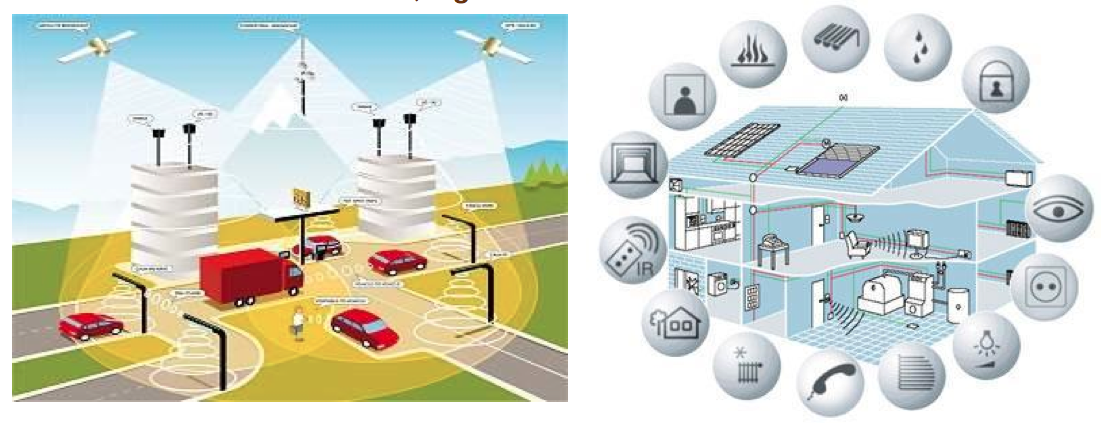
\includegraphics[width=14cm]{images/cenario_ubiquo.png}
  \caption[Ilustração de um cenário ubíquo]{Ilustração de um cenário ubíquo.}
  \label{fig:exampleFigCenarioUbiquo}
\end{center}
\end{figure}

Ainda de acordo com \cite{poslad2009}, existem três requisitos fundamentais na Computação Ubíqua que fora idealizada por Mark Weiser: computadores precisam estar distribuídos, interligados e acessíveis de forma transparente; a interação humano-computador deve ser escondida ou, simplesmente, minimizada; para que os sistemas possam otimizar suas operações nos diversos ambientes dinâmicos em que operam, esses precisam ser sensíveis ao contexto.  O autor ainda considera outros dois requisitos adicionais como sendo, também, fundamentais: computadores devem operar de maneira automática; computadores devem lidar com  múltiplas ações dinâmicas. 
	
Segundo \cite{lopes2011}, uma das principais características dos sistemas ubíquos são os ambientes altamente dinâmicos  nos quais estes estão inseridos. Para Lopes, nesses ambientes dinâmicos, diversos dispositivos, de natureza diferente ou não, interagem entre si com a finalidade de fornecer informações relevantes que, de algum modo, possa contribuir com as atividades cotidianas dos usuários de maneira imperceptível.
	
Isto posto, a computação ubíqua é a computação onipresente, isto é, acessível em todos os lugares, conforme apresentado na figura \figref{fig:exampleFigCenarioUbiquo}, que tem o propósito de facilitar a interação entre usuários e dispositivos computacionais espalhados pelo ambiente, de modo que esses usuários não percebam que estão fornecendo comandos para os computadores que os cercam.  Em outras palavras, é a computação por meio da comunicação entre usuários, dispositivos e ambientes, objetivando simplificar e, sobretudo, facilitar a realização das tarefas cotidianas dos usuários sem que estes percebam.


\section{Propriedades}
\label{sc:propriedades}
Hodiernamente, na literatura, podemos encontrar um grande número de requisitos da computação ubíqua. Todavia, para efetivamente caracterizar o ideal que fora criado por Weiser, pesquisadores espalhados por todo mundo documentam, em suas publicações acadêmicas, as propriedades essenciais para o verdadeiro cenário ubíquo \citep{gomes2007}. 

Esta seção tem o propósito de apresentar uma coleção dos requisitos mais relevantes da computação ubíqua. 

\subsection{Sensibilidade ao Contexto}
Uma das principais áreas de pesquisa dentro da computação ubíqua é a computação sensível ao contexto  \citep{carmo2012}. Segundo \cite{schilit1994}, o primeiro a apresentar uma definição para o termo, a computação sensível ao contexto é “\textit{o estudo de aplicações que se adaptam de acordo com a localização do usuário, grupo de pessoas, objetos próximos ao usuário e as mudanças ocorridas com esses objetos ao longo do tempo}”. A partir desse ponto, surgiram diversos conceitos, de diversos autores, mas sempre conceituando o termo de forma bastante semelhante:

\begin{itemize}
\item Aplicações que conseguem modificar ou adaptar seu comportamento dinamicamente baseado nas informações de contexto do usuário ou da aplicação \citep{ryan1997}.
\item Sistema que se utiliza de informações relativas ao contexto para fornecer, de alguma maneira, serviços ou informações relevantes ao usuário \citep{dey2000}.
\item Aplicações que se beneficiam da descoberta de informações de contexto tais como: localização do usuário, hora do dia, dia da semana, temperatura, dispositivos próximo ao usuário, etc. objetivando melhorar o desempenho de aplicações computacionais \citep{chen2000}.
\end{itemize}

Sabemos que Sistemas de Computação Ubíqua são integrados com o ambiente. Nesse sentido, esses sistemas precisam utilizar informações de contexto para proporcionar adaptações no comportamento e, sobretudo, nas funcionalidades do próprio sistema \citep{tandler2004}. Dessarte, essa característica permite não só que o sistema conheça o ambiente no qual está operando, mas que ele possa, também, se ajustar automaticamente de acordo com o contexto sem ao menos necessitar que o usuário esteja ciente desse ajuste.            

\subsection{Invisibilidade}
Muitos definem computação ubíqua também como computação invisível \citep{gomes2007}, e isso não é por acaso. Segundo \cite{weiser1991}, quanto mais uma tecnologia está presente em nossas vidas, menos perceptível ela se torna.  Nesta visão, o computador passa a se tornar fundamental na realização das principais atividades do dia-a-dia do usuário, todavia, dilui-se no mundo físico de tal forma que passa a se tornar, também, tão presente e imperceptível quanto o ar que se respira \citep{gomes2007}.

De acordo com \cite{queirozfilho2012}, esta propriedade pode ser interpretada em dois sentidos: o primeiro refere-se a miniaturização dos dispositivos computacionais, bem como a capacidade destes em se incorporar aos objetos do dia-a-dia (e.g. móveis, vestimentas, equipamentos médicos, etc.), tornando-se,  assim, fisicamente invisível para as pessoas;  a segunda interpretação refere-se a forma como os dispositivos conseguem trabalhar sem desviar a atenção do usuário e, por conseguinte,  tornando-os imperceptíveis.  Nesse sentido, apesar da tecnologia estar visível fisicamente ela consegue realizar duas funções sem necessitar da atenção dos usuários.  

\subsection{Interoperabilidade espontânea}
Em \cite{kindBerg2012}, os autores apontam a interoperabilidade espontânea como um das características fundamentais dos sistemas ubíquos. Além disso, eles afirmam que um sistema ubíquo é composto por componentes de infraestrutura e dispositivos computacionais heterogêneos que usam tecnologias diferentes, bem como oferecem funcionalidades diferentes e, portanto, a interoperabilidade espontânea é vista como uma característica desejável a implementação da computação ubíqua exatamente pelo fato da possibilidade de integração dinâmica entre esses componentes e dispositivos. 

Isto posto, a partir desta propriedade, dispositivos e serviços podem interagir de maneira automática e, sobretudo, sem intervenção do usuário, compartilhando recursos ou, simplesmente, trocando informações, permitindo, deste modo, uma completa integração entre os dispositivos espalhados pelo ambiente. 

Seja um ambiente ubíquo implementado em uma estação de ônibus de uma determinada cidade. A interoperabilidade espontânea pode ser observada se, por exemplo, o ônibus é capaz de transferir  para os usuários informações sobre horários, pontos e acontecimentos no seu percurso sem qualquer intervenção manual para configurar o dispositivo do usuário. Ou seja, a interoperabilidade espontânea  é caracterizada pela capacidade de um sistema se comunicar de forma transparente com outro sistema sem a necessidade de intervenção do usuário.


\subsection{Integração Física}
A integração física, assim como a interoperabilidade espontânea, é considerada uma das características fundamentais dos sistemas ubíquos \citep{kindBerg2012}. De acordo com \cite{gomes2007}, os espaços inteligentes, do inglês \textit{smart spaces}, se caracterizam pela intensa colaboração entre elementos computacionais e componentes do mundo físico. 
	
Com o objetivo de exemplificar tal integração,  \cite{kindBerg2012} citam o projeto denominado MediaCups \citep{mediacups2001}, onde uma xícara de café inteligente, além de servir como uma xícara de maneira usual, contém elementos como sensores, recursos de processamento e rede, que acabam permitindo que ela possa comunicar seu estado (e.g. cheio, vazio, frio, morno, etc.) ao seu proprietário. 
	
Nesse sentido, a integração física é justamente a ideia de que elementos computacionais se unam a componentes físicos rotineiramente utilizados pelas pessoas para que, através dessa colaboração, este conjunto possa trazer benefícios e, sobretudo, melhorar a interação com seu usuário.

\subsection{Adaptação e Tolerância a falhas}
Levando em consideração a grande dinamicidade existente na Computação Ubíqua, conforme já mencionado na seção \ref{sc:definicoes}, os sistemas ubíquos precisam adaptar suas configurações em tempo de execução para acompanhar ativamente as mudanças ocorridas no ambiente \citep{lopes2011}. Todavia, os sistemas precisam levar em consideração não somente as mudanças de contexto, mas, sobretudo, as falhas que podem ocorrer nos serviços disponíveis, na rede ou até mesmo nos dispositivos, bem como ter a capacidade de se adaptar, também, à essas falhas para que a parada ou travamento do sistema possa ser evitada.

Nesse sentido, essa capacidade de tolerar possíveis falhas fornece aos sistemas a possibilidade de manter o seu funcionamento exatamente como fora especificado mesmo mediante a ocorrência de falhas.     

\subsection{Interfaces naturais}
De acordo com \cite{gomes2007}, em \textit{smart-spaces}, faz-se necessário a busca por técnicas que permita a utilização de recursos comumente utilizados no dia-a-dia das pessoas, tais como  gestos, voz e até mesmo olhares como meio de comunicação entre homem e  máquina. Isto é, a ideia é exatamente levar elementos digitais ao mundo real, mas de maneira tão sutil que acaba não influenciando tanto na maneira como determinada atividade é realizada pelo usuário e, sobretudo, fazendo com que tal interação seja simples e natural.

\section{Contextos de Uso}
\label{sc:contextoDeUso}
Uma importante área de pesquisa dentro do domínio de dispositivos móveis é o que vem sendo denominado de contexto de uso \citep{carmo2012}. Este conceito tem como propósito trazer melhorias à experiência do usuário na utilização de dispositivos móveis.  

A ideia é coletar informações durante o uso do dispositivo, de maneira imperceptível para o usuário, que permita reconhecer o cenário atual.  Assim, ao identificar o contexto, é possível fornecer serviços que sejam de interesse para o usuário no momento e no cenário de uso e, por conseguinte, melhorar  sua experiência ao utilizar o dispositivo.

Em outras palavras, o objetivo é fazer com que um determinado dispositivo possa se adaptar às diversas situações de uso de modo a atender a necessidade do usuário no momento. Para exemplificar, suponhamos que um determinado usuário tenha o costume de correr todos os dias no parque ou na praia, e que quando ele está no parque gosta de ouvir um tipo de música diferente de quando ele está correndo na praia. Ao coletar informações de contexto referentes a atual localização do usuário,  o dispositivo poderia adaptar de forma automática sua interface, de modo que as músicas que o usuário costumeiramente escuta no local possa tocar no dispositivo. 

\section{Resumo do capítulo}
\label{sc:resumoUbicomp}

A computação sensível ao contexto é uma área da computação ubíqua em que as aplicações modificam ou adaptam seu comportamento com base nas informações coletadas do ambiente, para, desta forma, oferecer as informações que o usuário necessita. A coleta de informações se dá muitas vezes de forma imperceptível aos usuários.

Com o avanço dos recursos presentes nos dispositivos móveis, diversas aplicações surgiram para auxiliar o usuário nas suas tarefas diárias. Uma tarefa que tem causado transtornos à população das grandes cidades é a locomoção utilizando o transporte público. As informações fornecidas à respeito do transporte público não são suficientes e, na maioria das vezes, inúteis.

A ideia deste trabalho é, exatamente, criar uma aplicação mobile para prover informação aos usuários de transporte público, utilizando-se, para tanto, dos sensores existentes na maioria dos dispositivos móveis para fazer com que estes usuários, implicitamente, forneçam dados (localização, velocidade e etc.) para aplicação. Por exemplo, a aplicação proposta tem como objetivo permitir que os usuários colaborem com a divulgação sobre os principais acontecimentos no trânsito, mas, sabemos que nem todo mundo sabe a localização que se encontra, então a tarefa de cadastrar esse acontecimento no trânsito pode ser projetada de modo que o usuário não precise informar, explicitamente, sua localização, haja vista que esta pode ser obtida através dos sensores existentes no dispositivo.

Isto posto, a capítulo a seguir, além de apresentar uma técnica para solucionar problemas através do conhecimento coletivo denominada \textit{Crowdsourcing}, mostrando seus principais conceitos e definições, discute como as tarefas que envolvem colaboração podem ser projetadas a fim de diminuir o esforço do usuário, tornando-a mais simples, intuitiva e, por conseguinte, motivando estes usuários a colaborarem.